% Shared typography and palette for the research schematics.
\documentclass[tikz,border=9pt]{standalone}
\usepackage[T1]{fontenc}
\usepackage{lmodern}
\usetikzlibrary{arrows.meta,calc,positioning,backgrounds}
\renewcommand{\familydefault}{\sfdefault}
\hyphenpenalty=10000
\exhyphenpenalty=10000
\definecolor{Ink}{HTML}{263D4A}
\definecolor{Muted}{HTML}{536774}
\definecolor{Blue}{HTML}{24678E}
\definecolor{Teal}{HTML}{0D6B6E}
\definecolor{Green}{HTML}{26734D}
\definecolor{Gold}{HTML}{87641A}
\definecolor{PaleBlue}{HTML}{EDF4FA}
\definecolor{PaleTeal}{HTML}{ECF6F5}
\definecolor{PaleGreen}{HTML}{EFF6F0}
\definecolor{PaleGold}{HTML}{FAF5E9}
\definecolor{PaleGray}{HTML}{F2F5F6}
\tikzset{
  every node/.style={text=Ink,font=\sffamily\fontsize{11}{14}\selectfont},
  panel/.style={draw=#1!65,fill=#1!5,line width=.7pt,rounded corners=5pt,
    minimum width=5.7cm,minimum height=3.4cm,text width=4.95cm,
    inner sep=10pt,align=left,anchor=north west},
  flow/.style={-{Stealth[length=5pt,width=5pt]},draw=Muted,line width=1pt,
    shorten <=4pt,shorten >=4pt},
  note/.style={text width=11.8cm,align=left,font=\sffamily\fontsize{10}{13}\selectfont,
    text=Muted,anchor=north west},
}
\newcommand{\heading}[2]{
  \node[anchor=north west,text width=12.4cm,font=\sffamily\bfseries\fontsize{21}{25}\selectfont]
    at (0,1.9) {#1};
  \node[note] at (0,.85) {#2};
}
\newcommand{\panel}[6]{
  \node[panel=#4] (#1) at (#2,#3)
    {{\color{#4}\bfseries\fontsize{13}{16}\selectfont #5}\\[5pt]#6};
}
\newcommand{\fourflow}{
  \draw[flow] (a.east) -- (b.west);
  \draw[flow] (b.south) -- (c.north);
  \draw[flow] (c.west) -- (d.east);
}
\newcommand{\bottomnote}[1]{\node[note] at (0,-7.75) {#1};}
% Suppress volatile PDF metadata; SOURCE_DATE_EPOCH is also set by the builder.
\ifdefined\pdfinfoomitdate\pdfinfoomitdate=1\fi
\ifdefined\pdftrailerid\pdftrailerid{}\fi
\ifdefined\pdfsuppressptexinfo\pdfsuppressptexinfo=15\fi

\tikzset{
  sys/.style={font=\sffamily\bfseries\fontsize{12}{15}\selectfont,text width=3.3cm,align=left,anchor=north west},
  col/.style={font=\sffamily\bfseries\fontsize{11}{14}\selectfont,text=Muted,text width=4.2cm,align=center,anchor=north},
  cell/.style={draw=#1,fill=#1!5,line width=.8pt,rounded corners=4pt,
    minimum width=4.2cm,minimum height=2.1cm,text width=3.8cm,inner sep=6pt,
    align=left,anchor=north west,font=\sffamily\fontsize{10}{12.5}\selectfont},
  dev/.style={dashed,dash pattern=on 4pt off 3pt},
  chain/.style={draw=Ink!55,fill=PaleGray,line width=.7pt,rounded corners=4pt,
    minimum width=3.0cm,minimum height=1.9cm,text width=2.7cm,inner sep=5pt,
    align=center,font=\sffamily\bfseries\fontsize{10}{12.5}\selectfont},
}
\newcommand{\row}[3]{\node[sys,text=#2] at (0,#1) {#3};}
\begin{document}
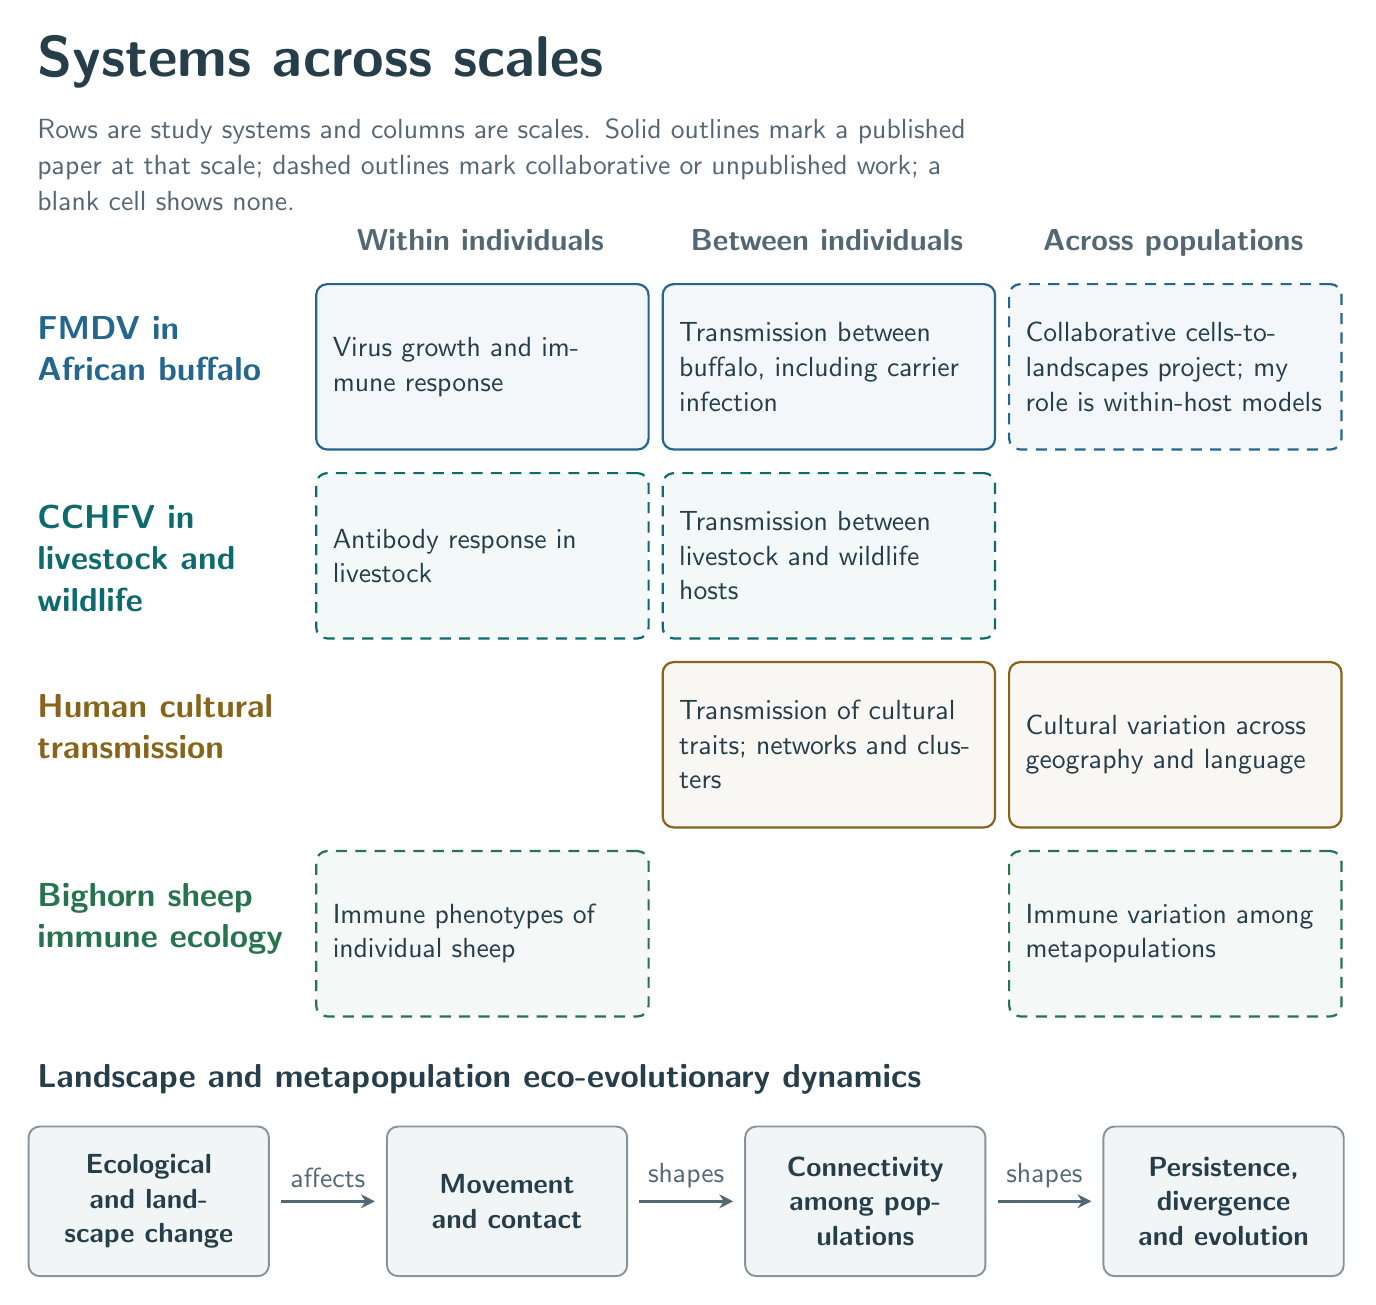
\begin{tikzpicture}
\heading{Systems across scales}{Rows are study systems and columns are scales. Solid outlines mark a published paper at that scale; dashed outlines mark collaborative or unpublished work; a blank cell shows none.}
% column headings
\node[col] at (5.75,-0.55) {Within individuals};
\node[col] at (10.15,-0.55) {Between individuals};
\node[col] at (14.55,-0.55) {Across populations};
% FMDV
\row{-1.65}{Blue}{FMDV in African buffalo}
\node[cell=Blue] at (3.65,-1.35) {Virus growth and immune response};
\node[cell=Blue] at (8.05,-1.35) {Transmission between buffalo, including carrier infection};
\node[cell=Blue,dev] at (12.45,-1.35) {Collaborative cells-to-landscapes project; my role is within-host models};
% CCHF
\row{-4.05}{Teal}{CCHFV in livestock and wildlife}
\node[cell=Teal,dev] at (3.65,-3.75) {Antibody response in livestock};
\node[cell=Teal,dev] at (8.05,-3.75) {Transmission between livestock and wildlife hosts};
% Culture
\row{-6.45}{Gold}{Human cultural transmission}
\node[cell=Gold] at (8.05,-6.15) {Transmission of cultural traits; networks and clusters};
\node[cell=Gold] at (12.45,-6.15) {Cultural variation across geography and language};
% Bighorn
\row{-8.85}{Green}{Bighorn sheep immune ecology}
\node[cell=Green,dev] at (3.65,-8.55) {Immune phenotypes of individual sheep};
\node[cell=Green,dev] at (12.45,-8.55) {Immune variation among metapopulations};
% chain
\node[anchor=north west,font=\sffamily\bfseries\fontsize{12}{15}\selectfont,text=Ink] at (0,-11.15) {Landscape and metapopulation eco-evolutionary dynamics};
\node[chain,anchor=north west] (s1) at (0,-12.05) {Ecological and landscape change};
\node[chain,anchor=north west] (s2) at (4.55,-12.05) {Movement and contact};
\node[chain,anchor=north west] (s3) at (9.1,-12.05) {Connectivity among populations};
\node[chain,anchor=north west] (s4) at (13.65,-12.05) {Persistence, divergence and evolution};
\draw[flow] (s1.east) -- node[above,font=\sffamily\fontsize{10}{12}\selectfont,text=Muted,yshift=1pt] {affects} (s2.west);
\draw[flow] (s2.east) -- node[above,font=\sffamily\fontsize{10}{12}\selectfont,text=Muted,yshift=1pt] {shapes} (s3.west);
\draw[flow] (s3.east) -- node[above,font=\sffamily\fontsize{10}{12}\selectfont,text=Muted,yshift=1pt] {shapes} (s4.west);
\end{tikzpicture}
\end{document}
